%=========================================================================
% (c) Michal Bidlo, Bohuslav Křena, 2008

% treba doinstalovat balik: texlive-epstopdf

%==============================================================================|
\chapter{Introduction}
Testing is used to~find bugs~(errors or other defects) in~software. By~finding bugs,
testing also provides quality assurance of~software. Software testing can be stated
as the~process of~validating and~verifying that a~computer software:
\begin{itemize}
	\item meets the~design and~development requirements,
	\item works as expected,
	\item is secure,
	\item and~that bugs are not present.
\end{itemize}

Fuzzing is a~type of~testing where a~goal is to~find bugs in~software, preferably
ones that have security implications. Fuzzing is automated, brute force technique
of~testing and~it exploits the~fact that many bugs in~software are caused
by~handling inputs from~a~user without applying validation routines on~that
inputs. The~goal of~fuzz testing~(fuzzing) is to~crash an~application or a~protocol
and~analyze the~results. Fuzzing is presented in~the~next chapter.\\

The goal of~this work is to~test applications using \mbox{D-Bus} communication
system and~to~implement a~tool for~automation of~this task. The targets of~testing
done in~this work are applications connected to~a~session bus daemon and~using it
for~routing messages.\\

In~the~third chapter the~D-Bus message bus system is described. The~chapter includes
description of~protocols in~general, D-Bus architecture, message bus daemons,
addressing on~D-Bus, calling methods and~emitting signals. Also the~GDBus \mbox{D-Bus}
binding is described which was used in~an~implementation of~the~fuzzing tool.\\

The~fourth chapter is devoted to~description of~designing a~tool for~fuzzing
applications using D-Bus communication system. The~chapter discusses methods
which can be used for~testing D-Bus system and its applications. Subsequently,
the~architecture of~the~tool for~fuzzing and~its implementation are described.\\

\newpage
Results of~the~fuzz testing performed with~the~implemented tool are discussed
in~the~fifth chapter. The~chapter includes tables where methods and~results
of~their calls are stated for~every tested application. Also the~run times
of~the~tests are stated and~for~the~tests where memory leaks were detected,
the~tables also contains a~normal process memory usage against an~abnormal one.\\

The~conclusion summarizes what was the~purpose of~this work, how a~fuzzing was used
to~test applications using \mbox{D-Bus} communication system, evaluation of~results
and~achievements and~suggestions for~improvements.



%==============================================================================|
\chapter{Fuzzing}
The~term fuzzing was first used by~professor Barton Miller who used fuzzing to~test
robustness of~UNIX applications in~1989~\cite{Fuzzing2}. Fuzzing is defined
in~``Fuzzing: Brute Force Vulnerability Discovery''~\cite[p.~22]{Fuzzing} as
``\emph{a~method for~discovering faults in~software by~providing unexpected
input and~monitoring for~exceptions. It is typically an~automated or semiautomated
process that involves repeatedly manipulating and~supplying data to~target software
for~processing}''.
Another definition~(from ``Fuzzing for~Software Security Testing and~Quality
Assurance''~\cite[p.~1]{Fuzzing2}) says it is ``\emph{a~highly automated testing
technique that covers numerous boundary cases using invalid data~(from~files,
network protocols, API calls, and~other targets) as application input to~better
ensure the~absence of~exploitable vulnerabilities. The~name comes~from modem
applications tendency to~fail due to~random input caused by~line noise on~`fuzzy'
telephone lines}''. Some other terms used to~describe tests similar to~fuzzing
include~\cite[p.~24]{Fuzzing2}:
\begin{itemize}
	\item Negative testing
	\item Protocol mutation
	\item Robustness testing
	\item Syntax testing
	\item Fault injection
	\item Rainy-day testing
	\item Dirty testing
\end{itemize}

The aim of~fuzzing is to~crash a~program or a~protocol and~analyze the~crash results.
This is why many vendors want a~crash data. It is very important because a~crash
tells so much about a~program. Fuzzing is close to~the~boundary value analysis, where
you create test values that infringe the~boundary of~known good and~bad values.
Fuzzing is very effective because many exploitable vulnerabilities are caused
by~applications accepting user input and~processing that data without applying
validation routines~\cite{Fuzzing}.\\

The~division of~fuzzers to~categories and~subcategories as~also information
gathered in~this chapter are from~books ``Fuzzing: Brute Force Vulnerability
Discovery''~\cite{Fuzzing} and~``Fuzzing for~Software Security Testing and~Quality
Assurance''~\cite{Fuzzing2}.


\section{Fuzzing as software testing technique}
Testing in~general uses two different approaches. The~``white box'' testing is used
to~test internal structures of~an~application as testers have access to~a~source code
of~an~application and~so are able to~test many conditions and~paths through the~code
base and~uncover potential errors. In~the~``black box'' approach testers do not have
a~knowledge of~an~application internals. Testers are aware of~what the~application is
supposed to~do but are not aware of~how it does it. Rather than internals
the~functionality of~an~application is tested and~the~same applies for~fuzzing
as it is essentially the~functional testing technique focused on~the~software
security. The~functional testing can be viewed as ``black box'' with~one or more
external interfaces available for~injecting test cases, but without any other
information available on~the~internals of~the~tested system.\\

One of a~fuzzing main goals is to~crash a~system. It is a~testing approach that
would almost never occure in~a~normal environment~(the~negative testing) and~it
is used to~test software robustness. As stated in~``Fuzzing for~Software Security
Testing and~Quality Assurance''~\cite[p.~18]{Fuzzing2} robustness of~software is
``\emph{an~ability to~tolerate exceptional inputs and~stressful environmental
conditions. Software is not robust if it fails when facing such circumstances.
Attackers can take advantage of~robustness problems and~compromise the~system
running the~software. Most security vulnerabilities reported in~the~public are
caused by~robustness weaknesses}''.\\

Programs and~frameworks that are used to~create fuzz tests or perform fuzz
testing are commonly called fuzzers. Fuzzers fit the~best for~finding errors that
can cause a~program to~crash, such as buffer overflows, denial of~service attacks,
format bugs and~SQL injections. Fuzz testing is less effective for~finding a~security
threats that do not cause program crashes, such as spyware, some viruses, worms,
trojans and keyloggers.\\

Fuzz testing is simple and~can often reveal defects that are overlooked when
software is designed, written and~debugged. Fuzz testing is usually used to~find
the~faults that a~normal testing is not able to~detect. As any other type
of~a~testing, fuzz testing also cannot guarantee a~complete security, quality
and~effectiveness of~software.


\section{Fuzzer categories} \label{sec:cat}
Fuzzers can be divided into~two groups:
\begin{itemize}
	\item \textbf{Mutation-based fuzzers} apply mutations on~existing data samples
	to~create test cases. This means that existing chunk of~data is taken by~a~fuzzer
	and~fields which are defined as modifiable by~specification within~this chunk are
	modified each time before sending that data to~the~tested software. Modifications
	can be random or driven by~some protocol specifications.
	\item \textbf{Generation-based fuzzers} create test cases from~scratch by~modeling
	the~target protocol of~a~certain format. Creating test cases includes use
	of~mechanisms to~generate valid data for~a~protocol or a~valid computer program
	for~a~compiler fuzz testing. Mechanisms to~generate such valid data can include
	finite state machines, formal grammars or formal languages.
\end{itemize}


\section{Fuzzer subcategories} \label{sec:subcat}
Generally we can divide fuzzers into~these subcategories:
\begin{itemize}
	\item pregenerated test cases
	\item random test cases
	\item manual protocol mutation testing
	\item mutation or brute force testing
	\item automatic protocol generation testing
\end{itemize}

\subsection{Pregenerated test cases}
This method was used in~\emph{PROTOS framework}~\cite{PROTOS}. The~method
includes studying a~particular specification to understand all supported data
structures and~the~acceptable value ranges. Packets or files are then generated
to~test boundary conditions or violate the~specification. A~disadvantage is that
there is no~random component, once the~list of~test cases is exhausted, fuzzing
is complete.

\subsection{Random test cases}
This method simply generate pseudo-random data and~uses it as~the~target input,
waiting for the~result. Example of~this can be:
\begin{lstlisting}[frame=single]
while [1]; do cat /dev/urandom | nc -vv localhost 22; done
\end{lstlisting}
This command reads random data from Linux urandom device and~then transmits
that data to~localhost address on~port~22~(ssh). The biggest disadvantage
of~this simple technique is tracking back how some random bytes caused
an~application crash. This includes capturing the~input we sent to~application
and~also debugging a~corrupted stack.

\subsection{Manual protocol mutation testing}
In~manual protocol mutation testing there is no~automated fuzzer involved.
The~researcher is the~fuzzer, simply entering inappropriate data in~an~attempt
to~crash an~application or to~find some undesirable behaviour. The success
depends on~the~researcher knowledge and experience. This class of~fuzzing is
most often applied to~web applications.

\subsection{Mutation or brute force testing}
A~brute force in~this class of~fuzzing is referring to~a~fuzzer that starts with
a~valid sample of~a~protocol or data and~continually mangles some amount
of~bytes within that data packet or file. It requires only a~little research
and~an~implementation of~a~brute force fuzzer is relatively straightforward.
The~main advantage is that the~process is fully automated. Disadvantages
are that it takes many samples of~data to~get decent coverage of~protocol
specifications or file definitions, so many CPU cycles will be wasted on~data
that cannot be interpreted. Examples of~brute force file format fuzzers include
\emph{FileFuzz}~\cite{FileFuzz} and~\emph{notSPIKEfile}~\cite{fuzzing.org}.

\subsection{Automatic protocol generation testing}
Automatic protocol generation testing is a~more advanced method of~brute force
testing. In~this approach, research is needed to~first understand a~protocol
specification and~a~file definition. Then the~grammar is created that describes
how the~protocol specification works. It includes identifying portions of~data
that are to~remain static and~others that represents fuzzable variables.
The~fuzzer then generates fuzz data for that variables and~sends the~resulting
packet to~the~target. The~success depends on~the~researcher's ability
to~pinpoint those portions of~the~specification that are most likely to~lead
to~faults in~the~target application. Examples of~this type of~fuzzers are
\emph{SPIKE}~\cite{Aitel} and~\emph{SPIKEfile}~\cite{fuzzing.org}.
Both of~these tools take \emph{SPIKE} script descriptions of~their
target protocol or file format and~use a~fuzzing engine of \emph{SPIKE}
framework to~create mangled data. \emph{SPIKE} is actually a~fuzzer creation
kit, providing an~API that allows users to~create their own fuzzers for~network
based protocols using the~C programming language. \emph{SPIKE} defines
a~number of~primitives that it makes available to~C coders which allows \emph{SPIKE} to~construct fuzzed messages called ``SPIKES'' that can be sent to~a~network
service to~hopefully induce errors.


\section{Fuzzer types} \label{sec:types}
Each type of~target has its own class of~fuzzer as~different target software
needs different approaches to~fuzzing. The~fuzzer types in~this section are
covering only basic types. There can be more different and~more specific fuzzer types.
Subsections in~this section will describe each type of~fuzzer
as~divided in~``Fuzzing: Brute Force Vulnerability Discovery''~\cite{Fuzzing}.

\subsection{Local fuzzers}
Local fuzzers are used for~fuzzing applications running on~the~same computer
and~operating system as local fuzzers do. They usually serve to~fuzz test command
line arguments, environment variables, and~any other locally available interfaces.
Interesting targets for~local fuzzers are UNIX setuid applications which allow
a~normal user to~temporarily gain elevated privileges. Any vulnerability in~this
type of~applications will give a~user escalated privileges and~ability to~execute
arbitary code. Example of~such an~application can be the~\texttt{passwd} program:
\begin{lstlisting}[frame=single]
ls -l --full-time /usr/bin/passwd
-rwsr-xr-x. 1 root root 27848 2012-12-04 18:27:43 +0100 /usr/bin/passwd 
\end{lstlisting}
which has the~setuid flag set, to~allow a~user to~change
a~password\footnote{in~``-rwsr-xr-x'' privileges string, the~``s'' letter means
a~file has the~setuid flag set}. Setuid means Set User ID upon execution.
If the~setuid flag is set on~a~file, a~user executing that file gets
the~permissions of~the~individual user or group that owns the~file. You can set
the~setuid flag of~a~file in~Linux by:
\begin{lstlisting}[frame=single]
sudo chown root:root file
sudo chmod u+s file
\end{lstlisting}
This will give a~user root privileges when executing the~file. There are two
distinct targets for~fuzzing setuid applications -- applications accepting
command-line arguments and~applications using environment variables.

\subsubsection{Command-line argument fuzzers}
Applications usually process command-line arguments as strings. The~following
example demonstrates command-line argument stack overflow:
\begin{lstlisting}[frame=single]
#include <string.h>
int main(int argc, char **argv) {
    char buffer[5];
    strcpy(buffer, argv[1]);
}
\end{lstlisting}
If it would have setuid bit set, it could be misused to~get elevated privileges.
The~easiest way to~find such errors~(even without source code available)
is fuzzing. Useful tools for command-line fuzzing can be
\emph{clfuzz}~\cite{clfuzz} and~\emph{iFUZZ}~\cite{fuzzing.org}
which can be used for~format string and~buffer overflow testing.

\subsubsection{Environment variable fuzzers}
Another local fuzzer type is a~fuzzer testing environment variables. Example
of~an~error where value from~the~environment variable \texttt{HOME} is used unsafely:
\begin{lstlisting}[frame=single]
#include <string.h>
int main(void) {
    char buffer[5];
    strcpy(buffer, getenv("HOME"));
}
\end{lstlisting}
This is the~similar error as~for command-line arguments -- the~buffer overflow.
Tools for fuzzing this type of~bugs are
\emph{Sharefuzz}~\cite{Aitel} and~\emph{iFUZZ}~\cite{fuzzing.org}.

\subsection{File format fuzzers}
Many applications are working with~file input and~output. All applications which
use configuration files need to~parse them. These applications must properly handle
file parsing even if files are malformed~(maliciously or by~some random damage).
The~file format fuzzers are used to~test these applications which must properly
handle file input. A~file format fuzzer will dynamically create different malformed
files that are then parsed using the~target application. The~examples of~useful
tools for~file fuzzing are \emph{notSPIKEfile}~\cite{fuzzing.org} and~\emph{SPIKEfile}~\cite{fuzzing.org}.

\subsection{Remote fuzzers}
Remote fuzzers are used for~testing software that listens on~a~network
interface. As most attacks are done remotely and~can provide an~attacker
with~access to~sensitive data, targeting these applications for~testing is
important. Targets for~this type of~fuzz testing include network protocols, web
applications and~web browsers.

\subsubsection{Network protocol fuzzers}
Network protocol fuzzers can be divided into~two categories based on~protocol
complexity. Simple protocols often have simple authentication or no authentication
at~all. They are usually based on~ASCII text and~do not contain checksum or length
fields. Complex protocols, on~the~other hand are comprised of~binary data and~they
might use encryption for~authentication. Useful tools for~network protocol fuzzing
are \emph{SPIKE}~\cite{Aitel} or \emph{Peach fuzzer}~\cite{Peach}.

\subsubsection{Web application fuzzers}
As web applications became popular they are used to~access back-end services
as e-mail, internet banking, and many more. Even traditional desktop applications
as word processing are available on~the~Web. Web application fuzzers must be capable
of~communicating via HTTP protocol and~they are looking for~vulnerabilities
unique to~specific Web applications. Example of~web application fuzzer is
\emph{WebScarab}~\cite{WebScarab} which behaves as a~proxy intercepting web
browser web requests and~web server replies.

\subsection{In-memory fuzzers}
In-memory fuzzers can be implemented by~freezing and~taking a~snapshot
of~a~process and~rapidly injecting faulty data into~one of~its input routines.
After each test case, the~snapshot taken previously is restored and~new data is
injected. This is repeated until all of~the~test cases are exhausted.

\subsection{Fuzzer frameworks}
A~fuzzing framework is a~generic fuzzer or fuzzer library that simplifies data
representation for~many types of~targets. Fuzzing framework usually includes
a~library to~produce fuzz strings or values that produce problems in~parsing
routines. It should also include a~script-like language for~creating a~specific
fuzzer. The~most important property of~generic fuzzers is reusability. The~main
disadvantages are development time of~a~framework, its complexity and~sometimes
limitations~(target of~fuzzing is not suitable for~framework). Fuzzing
frameworks include \emph{SPIKE}~\cite{Aitel} and~\emph{Peach fuzzer}~\cite{Peach}.



%==============================================================================|
\chapter{D-BUS}
D-Bus is a~protocol and~a~message bus system providing applications a~simple way
to~talk to~one another. D-Bus is ``\emph{a~system for~\mbox{inter-process}
communication~(IPC) and~makes it simple and~reliable to~code a~`single instance'
application or daemon, and~to~launch applications and~daemons on~demand when their
services are needed}''~\cite{DBUS}.\\

The~low-level API for~D-Bus is written in~C but most
of~the~documentation and~code is written for~a~higher level binding~(Python or GLib).
D-Bus has both the~system bus daemon (for~events such as ``new hardware device
added'' or ``printer queue changed'') and~the~session bus daemon (for~general
inter-process communication needs among user \mbox{applications}). The~message bus
is built on~top of~a~general one-to-one message passing framework, which can be
used by~any two applications to~communicate directly~(without going through
the~message bus daemon). The~communicating applications are either on~one computer,
or they communicate through unencrypted TCP/IP socket suitable for~use behind
a~firewall~\cite{DBUS}.\\

The source of~information in~this chapter was ``D-Bus specification''~\cite{DBUSspec},
``D-Bus tutorial''~\cite{DBUStutorial} and~``Red Hat Magazine''~\cite{DBUSrh}.


\section{Protocols}
Computers use protocols in~all aspects of~internal and~external communication.
Protocols represent a~structure for~data transfer and~processing with~defined
syntax. Certain standards and~rules understood by~both sending and~receiving
entities must be agreed on~to~communicate data in~meaningful way~\cite{Fuzzing}.\\

Some protocols are designed to~be human readable and~are represented in~plain
text form. Other protocols are represented in~binary format.

\subsubsection{Plain text protocols}
These protocols are human readable, they use mostly the~printable ASCII scheme.
This includes numbers, lowercase and~capital letters, symbols, carriage
returns~(\verb|'\r'|), new lines~(\verb|'\n'|), tabs~(\verb|'\t'|) and~spaces.
Plain text protocols are less efficient than binary protocols as~they are more
memory consuming, but they are easy to~debug and~analyse~\cite{Fuzzing}. Many
plain text protocols are transported in~serialised XML or JSON formats.

\subsubsection{Binary protocols}
Binary protocols consist of~a~stream of~raw bytes. Without an~understanding
of~the~protocol, the~packets will not be meaningful~\cite{Fuzzing}. They are
intended or expected to~be read by~a~machine rather than a~human being, as
opposed to~a~plain text. Binary protocols have advantage of~terseness, which
apply to~a~speed of~transmission and~interpretation. Binary protocols include
TCP, UDP, RTP or SSH.


\section{D-Bus architecture}
D-Bus has several layers:
\begin{itemize}
	\item A~library, \texttt{libdbus}, that allows two applications to~connect
		to~each other and~exchange messages.
	\item A~message bus daemon executable, built on~\texttt{libdbus},
		that multiple applications can connect~to. The daemon can route messages
		from~one application to~zero or more other applications.
	\item Wrapper libraries or bindings based on~particular application frameworks.
\end{itemize}


\begin{figure}[h]
\centering
\caption{D-Bus overview~\cite{DBUS}}
\label{fig:dbus_image}
\includegraphics[width=1\textwidth]{fig/dbus_diagram.eps}
\end{figure}


D-Bus contains the~bus daemons which act as~routers for~messages. Processes
can connect to~the~bus daemons to~use their routing services as stated on~D-Bus
overview~\ref{fig:dbus_image}. There are two standard buses: the~system bus
and~the~session bus.\\

The~system bus is a~global daemon that any application running in~any
context can use as~a~transport router. It is a~single point where applications
can export services that anyone can use. Only one system bus daemon
can be run at a~time within~an~operating system.\\

The~session bus is the~bus local to~the~current user's session. It is used
for~communication between applications running within the~same X~Window System\footnote{X~Window is a~system and~a~network protocol that provides a~basis
for~graphical user interfaces} session. For every login to~X, a~session bus
daemon is started.\\

D-BUS protocol is binary, which means D-BUS messages incur low overhead when
marshaling and~demarshaling data. Messages consist of~two sections, the~header
and~the~body. The~header contains routing information and~the~type signature
for~the~data. The body contains the~data being sent in~binary format. Each
piece~of~data has a~type code \mbox{associated} with~it and~is packed into the~body
accordingly. Some common types include bytes, 32 and~64 bit integers, doubles,
unix file descriptors and~strings. Common data types can be used to~build more
complex data~types such as arrays, dictionaries or structures.

\subsection{Objects and~object paths}
Messages are sent to~objects. A~D-Bus objects are conceptually similar to~those
found in~object oriented programming languages with~the exception that they are
pointed to~by~object paths~(not by~memory addresses). Object paths are in~forms
of~strings similar to~Unix file system paths. D-Bus exports
the~\texttt{/org/freedesktop/DBus} object. Applications can register as~many
objects as~they wish.

\subsection{Methods and~signals}
Each object has members -- methods and signals. Methods are operations that can
be invoked on~an~object, with~optional input~(arguments) and~output~(return values).
Signals are broadcasts from~the~object to~any application on~the~same bus, which
registered that it is interested in~signals emitted by~this object. Signals may
contain a~data payload. Methods and~signals are referred to~by~name.

\subsection{Interfaces}
Each object supports one or more interfaces. An~interface is a~named group
of methods and~signals~(as in GLib or Qt). Interfaces allow the~same method name
to~be used more than once, so the~interface is specifying which of~those methods
is actually invoked. Interfaces define the~type~of~an~object instance. D-Bus
identifies interfaces with~a~simple namespaced string.
Most bindings to~other programming languages have mapping of~those interface names
directly to~the~appropriate programming language constructs~(C++ virtual classes
for~example). D-Bus imports the~\texttt{org.freedesktop.DBus} interface.

\subsection{Proxies}
A~proxy object represents a~remote object in~another process. In the~low-level
D-Bus~C API it is necessary to~manually create a~method call message, send it,
then manually receive and~process the~method reply message.
In~higher-level bindings proxies are used to~do that instead.
So~when a~method is invoked on~a~proxy object, the~high-level binding converts it
into~a~D-Bus low-level method call message, waits for the~reply message, unpacks
the~return value, and returns it from~the~native D-Bus method.

\subsection{Bus names}
When each application connects to~the~bus daemon, the~daemon immediately assigns
it a~name, called the unique connection name. This unique name begins with a~colon
character. Bus daemon ensures that these unique names are never reused during
the~lifetime of~the~bus daemon, so~given unique name will always refer to~the~same
application. An~example of~a~unique name might be \texttt{:1.396}. The~numbers
after the~colon have no~meaning besides that they must be unique within the~bus
daemon. Application starts to~own a~name on~the~bus daemon as~soon as~the~name
is mapped to~a~particular application connection.\\

Applications may also own additional well-known names~(also called services).
A~\mbox{D-Bus} application may register one or more well-known names~(services)
that it will then own until it releases them. Example could be the~name called
\texttt{org.freedesktop.dfuzzer}.\\If application wants to~own this well-known
name~(service), it should have an~object at~the~path
\texttt{/org/freedesktop/dfuzzerObject}. This object must be supporting
the~interface \texttt{org.freedesktop.dfuzzerInterface}. Other applications
connected to~the~same bus daemon could then send messages to~this bus
name~(service), object and interface to~execute method calls.\\

In~general, the~unique names can be thought of~as IP addresses and~the well-known
names as domain names. So \texttt{org.freedesktop.dfuzzer} might map to~something
like \texttt{:1.396} just as \texttt{google.com} maps to~IP address
\texttt{173.194.35.70}.\\

Using well-known names~(services) brings one big advantage. When an~application
crashes or exits, the~operating system kernel has a~responsibility to~close
its connection to~the~message bus. As~soon as~the~message bus daemon registers
that an~application disconnected, it sends out notification messages to~all remaining
applications that the~disconnected application names have lost their owner.
This can be used by~other applications to~monitor the~lifetime of~an~application
in~which they are interested or an~application they communicate with.

\subsection{Addresses}
Applications which use D-Bus are either servers or clients. A~typical server
would be the~bus daemon which listens for~incoming connections. Client on~the~other
hand initiates a~connection to~the~server~(typically the~bus daemon) and~when
the~connection is established, communication is a~symmetric flow of~messages. Using
client-server architecture only matters when~setting~up connections.\\

A~D-Bus address specifies where a~server will listen to~connections, and~where
a~client will connect. An~example could be the~address \texttt{unix:path=/tmp/abcdef}
which specifies that the~server will listen on~a~UNIX domain socket at~the~path
\texttt{/tmp/abcdef} and~the~client will connect to~that socket. An~address
of~a~server can also specify TCP/IP sockets or any other transport mechanism.\\

The~address of~the~session bus daemon can be determined by~reading
an~environment variable -- in~D-Bus protocol, this is done by~\texttt{libdbus}
automatically. \texttt{libdbus} also discovers the~system bus daemon
by~checking a~well-known UNIX domain socket path~(an~environment variable can be
also used for~the~system bus daemon discovery).\\

In~an~unusual case when not using a~bus daemon, there is a~need to~define
client-server architecture -- who will be the~server and~who will be the~client.
Also a~mechanism for~them to~agree on~the~server address must be specified.\\

\subsection{Calling a~method}
To make a~particular method call on~a~particular object instance, a~number
of~nested components have to~be named:\\

			\texttt{Address -> [Bus Name] -> Path -> Interface -> Method}\\

The~bus name is optional~(in~brackets), as you only use it to~route the~method
call to~the~right application when using the~bus daemon. Otherwise a~direct
connection is used, so bus names are not used as there is no bus daemon.\\

The interface is used primarily for historical reasons, but it should be used
anyway. If the interface is omitted, a method name is ambiguous and it is
undefined which method will be invoked. When calling a~method, two messages are
routed through the~bus daemon:
\begin{itemize}
	\item a~method call message sent from~process \texttt{A} to~process \texttt{B}
	\item a~matching method reply message sent from~process \texttt{B} to~process \texttt{A}
\end{itemize}
The~caller includes a~different serial number in~each call message, and~the~callee
includes this number to~allow the~caller to~match replies to~calls.\\

D-Bus methods may accept any number of~arguments and~may return any number
of~values, including none. When method calls specify no return value,
a~``method return'' message is still sent to~the~calling application. This
allows applications using the~remote API to~know that the~remote method invocation
has completed even if no useful result is returned.\\

The~only way to~suppress the~generation of~the~reply message in~an~acknowledgement
to~a~D-Bus method call is if the~``no reply expected'' flag is sent as part
of~the~method invocation. It is an~optional D-Bus implementation feature.

\subsection{Emitting a~signal}
A~signal in~D-Bus consists of~a~single message, sent by~one process to~any
number of~other processes and~is entirely asynchronous. Signals may be emitted
by~D-Bus objects at~any time. A~signal is an~unidirectional broadcast and~it may
contain only arguments~(a~data payload), as it is a~broadcast, so it never has
a~return value.\\

The~emitter~(sender) of~signals sends them to~the~bus daemon. Recipients
of~the~signals register within~the~bus daemon to~receive signals based on~match
rules -- these rules typically include the~sender and~the~signal name.
The~bus daemon then sends signals only to~those recipients who have registered
them.\\


\section{GDBus -- GLib D-Bus binding}
Bindings are used to~wrap low-level D-Bus C API calls to~the~higher level
libraries or language constructs. Whenever the~low-level D-Bus API is changed,
only internals of~bindings must be modified. This protects all of~the~applications
using these bindings against need to~adapt their code whenever D-Bus protocol is
changed. That was the~main reason why GDBus binding was used for~implementation
of~the~tool for~fuzz testing applications using D-Bus system. Binding to~GLib was
chosen because many applications use it already and~it is also the~main higher level
binding for~GNOME applications communicating through \mbox{D-Bus} system.\\

The~source of~information in~this section was ``GNOME Developer Center''
and~its documentations~\cite{GNOMElow, GNOMEhigh}.\\

\subsection{Connection to~a~message bus}
The~\texttt{GDBusConnection} type is used for D-Bus connections to~remote peers
such as a~message buses. It is a~low-level API which provides methods
for~connection to~the~specified message bus and~also setting up connection
properties. When a~connection is established, the~\texttt{GDBusConnection} type
holds information about it.

\subsection{Proxy for~accessing D-Bus interfaces}
For~creating a~proxy, the~\texttt{GDBusConnection} type, a~bus name~(well-known
or unique), an~object path and~a~D-Bus interface name are required. If a~proxy is
created for~a~well-known name and~no name owner currently exists, the~message bus
will be requested to~launch a~name owner for~the name. This means that if
an~application requesting some well-known name~(service) creates a~proxy for~that
well-known name~(and no name owner currently exists), a~name owner will be launched
by~message bus. On~successful proxy creation, it will be stored
in~\texttt{GDBusProxy} base class, which could be then used to~access a~D-Bus
interface on~a~remote object for~calling methods or emitting signals.

\subsection{Object introspection}
Object introspection can be used to~obtain information about object interfaces,
interface methods and~individual method parameteres. The~introspection file can
be obtained by~calling the~\texttt{org.freedesktop.DBus.Introspectable.Introspect} method on~an~initialized proxy base class. This method name contains dots to~let
D-Bus know that a~name is split into~interface and~method name parts. This allows
using proxy for~invoking methods on~other interfaces.
Call of~the~\texttt{org.freedesktop.DBus.Introspectable.Introspect} method returns
introspection of~object in~serialized form in~a~\texttt{GVariant} type.
\texttt{GVariant} value is then deserialized into~classical string, which is
parsed and~output of~parsing is used to~fill a~\texttt{GDBusNodeInfo} structure.
This structure can be then used to~find desired interfaces, methods and~arguments
either by~specialized GDBus functions or by~working with pointers through
a~\texttt{GDBusNodeInfo} structure. Example of~introspection
of~the~\texttt{/org/gnome/Shell} object by~calling tool for~working with~D-Bus
objects, \texttt{gdbus}~(some omitted iterfaces are highlighted by~dots):
\begin{verbatim}
$ gdbus introspect --session -d org.gnome.Shell -o /org/gnome/Shell --xml

<!DOCTYPE node PUBLIC "-//freedesktop//DTD D-BUS Object Introspection 1.0//EN"
    "http://www.freedesktop.org/standards/dbus/1.0/introspect.dtd">
<!-- GDBus 2.34.2 -->
<node>
  .
  .
  .
  <interface name="org.freedesktop.DBus.Introspectable">
    <method name="Introspect">
      <arg type="s" name="xml_data" direction="out"/>
    </method>
  </interface>
  .
  .
  .
  <interface name="org.gnome.Shell">
    <method name="Eval">
      <arg type="s" name="script" direction="in">
      </arg>
      <arg type="b" name="success" direction="out">
      </arg>
      <arg type="s" name="result" direction="out">
      </arg>
    </method>
    <method name="ScreenshotArea">
      <arg type="i" name="x" direction="in">
      </arg>
      <arg type="i" name="y" direction="in">
      </arg>
      <arg type="i" name="width" direction="in">
      </arg>
      <arg type="i" name="height" direction="in">
      </arg>
      <arg type="b" name="flash" direction="in">
      </arg>
      <arg type="s" name="filename" direction="in">
      </arg>
      <arg type="b" name="success" direction="out">
      </arg>
    </method>
    <method name="ScreenshotWindow">
      <arg type="b" name="include_frame" direction="in">
      </arg>
      <arg type="b" name="include_cursor" direction="in">
      </arg>
      <arg type="b" name="flash" direction="in">
      </arg>
      <arg type="s" name="filename" direction="in">
      </arg>
      <arg type="b" name="success" direction="out">
      </arg>
    </method>
    <method name="Screenshot">
      <arg type="b" name="include_cursor" direction="in">
      </arg>
      <arg type="b" name="flash" direction="in">
      </arg>
      <arg type="s" name="filename" direction="in">
      </arg>
      <arg type="b" name="success" direction="out">
      </arg>
    </method>
    <method name="FlashArea">
      <arg type="i" name="x" direction="in">
      </arg>
      <arg type="i" name="y" direction="in">
      </arg>
      <arg type="i" name="width" direction="in">
      </arg>
      <arg type="i" name="height" direction="in">
      </arg>
    </method>
    <property type="b" name="OverviewActive" access="readwrite">
    </property>
    <property type="s" name="ShellVersion" access="read">
    </property>
  </interface>
  .
  .
  .
</node>
\end{verbatim}

As seen from~object introspection, the~\texttt{/org/gnome/Shell} object has more
interfaces~(object must have at~least one interface). Interfaces has methods
and~signals. Each argument of~a~method is declared with~name, its direction
and~signature string~(signature encodings are in~table~\ref{tab:tab1}).

\subsection{Method calls}
To~call a~method, its name must be specified including arguments serialized
in~a~\texttt{GVariant} type. Each argument of~a~method has its signature encoding
as stated in~table \ref{tab:tab1}.\\

\FloatBarrier
\begin{table}[!h]
\catcode`\-=12
\caption{Signature encoding}
\label{tab:tab1}
\begin{center}
	\begin{tabular}{| l | l |}
	\hline
	\textbf{Character} & \textbf{Data type} \\ \hline
	y & 8-bit unsigned integer \\ \hline
	b & boolean value \\ \hline
	n & 16-bit signed integer \\ \hline
	q & 16-bit unsigned integer \\ \hline
	i & 32-bit signed integer \\ \hline
	u & 32-bit unsigned integer \\ \hline
	x & 64-bit signed integer \\ \hline
	t & 64-bit unsigned integer \\ \hline
	d & double-precision floating point number \\ \hline
	s & UTF-8 string (no embedded null characters) \\ \hline
	o & D-Bus Object Path string \\ \hline
	g & D-Bus Signature string \\ \hline
	a & Array \\ \hline
	( & Structure start \\ \hline
	) & Structure end \\ \hline
	v & Variant type (GVariant type) \\ \hline
	\{ & Dictionary begin \\ \hline
	\} & Dictionary end \\ \hline
	h & Unix file descriptor \\
	\hline
	\end{tabular}
\end{center}
\end{table}
\FloatBarrier

The~signatures of~arguments are then joined to~form the~signature
string, which serves as format string~(similar to~the~format strings
in~\texttt{printf()} function) to~create a~\texttt{GVariant} type containing
all argument values. For example, a~method accepting a~string and a~signed
\mbox{32-bit} integer and returning no values would use ``\texttt{(si)}''
for~the~argument signature and~empty string for~the~return value.

\subsection{Using \texttt{GError}}
GLib provides a~standard method of~reporting errors from a~called function
to~the~calling code. Reporting errors is solved by~exceptions in~many other
languages. Almost every function takes a~return location of~\texttt{GError}
object as its last parameter. Caller of~the~function can then~(after a~function
return) test a~\texttt{GError} value if it is not \texttt{NULL}, report error
message to~a~user and~recover from~the~error or end a~program.



%==============================================================================|
\chapter{Designing dfuzzer, a~tool for~fuzz testing processes using D-Bus system}
There are many ways of~fuzz testing D-Bus system. In~general there are two main
possibilities:
\begin{itemize}
	\item fuzz testing of~the~D-Bus daemons and~the~D-Bus protocol
	\item fuzz testing of~D-Bus daemons clients
\end{itemize}


\subsubsection{Fuzz testing of the~D-Bus daemons and~the~D-Bus protocol}
When fuzz testing the~D-Bus daemons and~its protocol there is need to~use the~native
C \mbox{D-Bus} API. Bindings cannot be used, because they have strict checks
of~data being sent through their proxy objects. The~principle of~this
fuzz testing would be communication of~two applications through a~D-Bus daemon.
They would send malformed D-Bus protocol packets~(messages) to~each other,
by~mangling portions of~data within~these packets. Fuzzer would have to~simulate
a~communication between bus daemon clients and~it would also have to~be
watching the~bus daemon status -- its memory usage and~its state.


\subsubsection{Fuzz testing of~D-Bus daemon clients}
This work was considering three options of~fuzz testing D-Bus clients:
\begin{itemize}
	\item Connect to~the~session bus daemon and~test processes connected to~it
		by~sending them messages and~monitoring results
	\item Connect to~the~system bus daemon and~test processes connected to~it
		by~sending them	messages and~monitoring results
	\item Simulate the~session bus daemon, let processes connect and~test them
\end{itemize}

The first two options -- using the~session/system bus daemon for~routing messages
between processes has many advantages. The~biggest one is that all processes
connected to~a~bus and~using well-known names can be fuzz tested. This is
enabled by~an~object introspection. The~object introspection tells what interfaces
does the~object contain, including interface methods and~their arguments. Other
advantages may be routing of~messages by~a~bus daemon or using bindings instead
of~the~native D-Bus C API, which is related to~produce less code. Disadvantage
of~using the~session/system bus daemon with~bindings are strict data checks, which
do not allow to~route undesirable messages as for~example invalid UTF-8 strings
or object paths. Although it may seem to~be a~limitation for~a~fuzzer, other
processes using bindings have this limitation too, so it would not be appropriate
to~test messages the~processes can never send or receive through a~bus daemon.\\

The third option -- simulating session bus daemon would require using the~native C
D-Bus API with~\texttt{libdbus} library. This includes to~code a~bus daemon simulator
which can handle D-Bus connections and~use message dispatcher with~destination
table to~correctly route messages through D-Bus connections between processes.
Fuzz testing would then include connection of~tested processes to~the~bus daemon
simulator and~letting them communicate with~each other. The~bus daemon simulator
would be modificating this communication messages and~watching processes reactions
to~these modificated messages.\\

The~first option was chosen for~the fuzzer as there are more applications
on~the~session bus than on~the~system bus daemon and~there is no need to~implement
the~tool in~the~native D-Bus C API. The~system bus daemon also uses the~same
mechanism for~connection of~applications as the~session bus, and~so extending
the~fuzzer to~work also for~the~system bus daemon should be straightforward.


\section{dfuzzer architecture}
dfuzzer is a~tool implemented within~this work for~testing D-Bus applications.
Targeted applications for~dfuzzer are session bus daemon clients. It is
a~command-line tool which takes options as arguments for~setting~up fuzz testing
of~a~chosen application. dfuzzer is a~generation-based fuzzer~(\ref{sec:cat})
and~it randomly generates data for~method arguments according
to~signatures of~arguments~(\ref{tab:tab1}). It is a~local fuzzer~(\ref{sec:types})
although it does not interact with~tested applications processes directly, but
through a~system daemon -- the~session bus.

\subsubsection{Division into modules}
dfuzzer is using a~modular architecture, and~so individual problems are divided
into~individual modules. These modules include \emph{random module},
\emph{introspection module} and~\emph{fuzz module}.\\

The~\emph{random module} is responsible for~pseudo-random data generation. It can
generate data for~every primitive method argument signature~(\ref{tab:tab1}), except
complex data types as structures, arrays of~types and~dictionaries which were
not implemented. It also saves generated data sizes to~be able to~give a~condition
to~end fuzz testing of~a~method.\\

The~\emph{introspection module} performs an~object introspection. It requests
introspection file of~a~chosen object from~the~session bus daemon. Returned XML file
with~object interfaces, methods and~their arguments is then parsed into~GDBus
structures and~desired interface is found. The~\emph{introspection module} also
includes iterators for~these GDBus structures to~\mbox{iterate} through interface
methods and~their arguments.\\

The~\emph{fuzz module} is given a~name of~a~method and~its arguments signatures.
Subsequently, individiual arguments are created from~the~signatures
by~the~\emph{random module} for~data generation. After arguments were created,
a~method is called. When a~method call returns \texttt{NULL}, it means that a~tested
application does not respond or it disconnected from~the~bus daemon.
The~\emph{fuzz module} is also parsing a~\texttt{/proc/pid/status}\footnote{pid is process identification number} file to~monitor a~tested application process status
to~be able to~confirm that a~tested application really disconnected from~the~bus
daemon. Process status file is also used for~monitoring an~application process
memory usage.\\


\section{dfuzzer implementation}
The~tool for~fuzzing session bus clients was implemented in~the~C
programming language using GDBus binding to~the~native D-Bus C~API. The~fuzzer was
implemented and~tested in~the~GNU/Linux operating system.\\

When a~user logs in~to~X Window System, the~session bus daemon is started. Application
processes can then connect to~the~session bus daemon to~use it
for~an~\mbox{inter-process} communication. When a~process is connected to~the~session
bus, it can either provide a~sevice~(specified by~well-known name) or only use
the~session bus daemon for~communication with~other processes. Usually a~process
with~a~well-known name acts as a~server and~a~process with~a~unique name is
initiating a~connection and~so acts as a~client.\\

dfuzzer is fuzz testing only processes with~well-known names on~the~session bus
daemon. This means it needs to~own only a~unique name within~the~session bus.
dfuzzer is a~command-line tool which takes the~following required options as its
arguments:

\begin{itemize}
	\item a~process bus name
	\item a~process object path
	\item a~process interface
\end{itemize}

These options are required as dfuzzer must know which interface of~which object
and~which bus name it should communicate with~through the~session bus daemon.
Other options which are not required include:

\begin{itemize}
	\item a~name of~a~file for~logging~(default created log file is \emph{log.log})
	\item memory limit for~a~tested process -- if this limit is exceeded,
		dfuzzer logs a~warning message into~a~log file~(default memory limit
		was chosen as three times process initial memory size)
	\item maximum buffer size for~generated strings~(default maximum size
		is 50000~bytes)
	\item flag to~launch process after crash -- if tested process crashes during
		fuzzing and~this option is set, crashed process will be launched again
		and~testing will continue
\end{itemize}

When dfuzzer is launched it creates a~connection to~the~session bus daemon
by~calling the~method \texttt{g\_bus\_get\_sync()} which returns
a~\texttt{GDBusConnection} object containing all information about the~connection
including unique name assigned to~dfuzzer from~the~session bus daemon. Then
a~specified process bus name, an~object path and~an~interface are used in~call
of~the~function \texttt{g\_dbus\_proxy\_new\_sync()} to~create a~\texttt{GDBusProxy}
object which will be used for~communication with~a~tested process. Communication
of~dfuzzer with~a~tested process is shown on~the~figure~\ref{fig:dfuzzer_image}.
After connecting to~the~session bus \mbox{daemon}, dfuzzer requests a~tested process
identifier for~a~specified process bus name by~calling the~method
\texttt{org.freedesktop.DBus.GetConnectionUnixProcessID}. A~process identifier
is used for~monitoring a~tested process status.\\


\begin{figure}[h]
\centering
\caption{dfuzzer communication with~\emph{GNOME Shell}~\cite{GNOMEShell}
		through the~bus daemon}
\label{fig:dfuzzer_image}
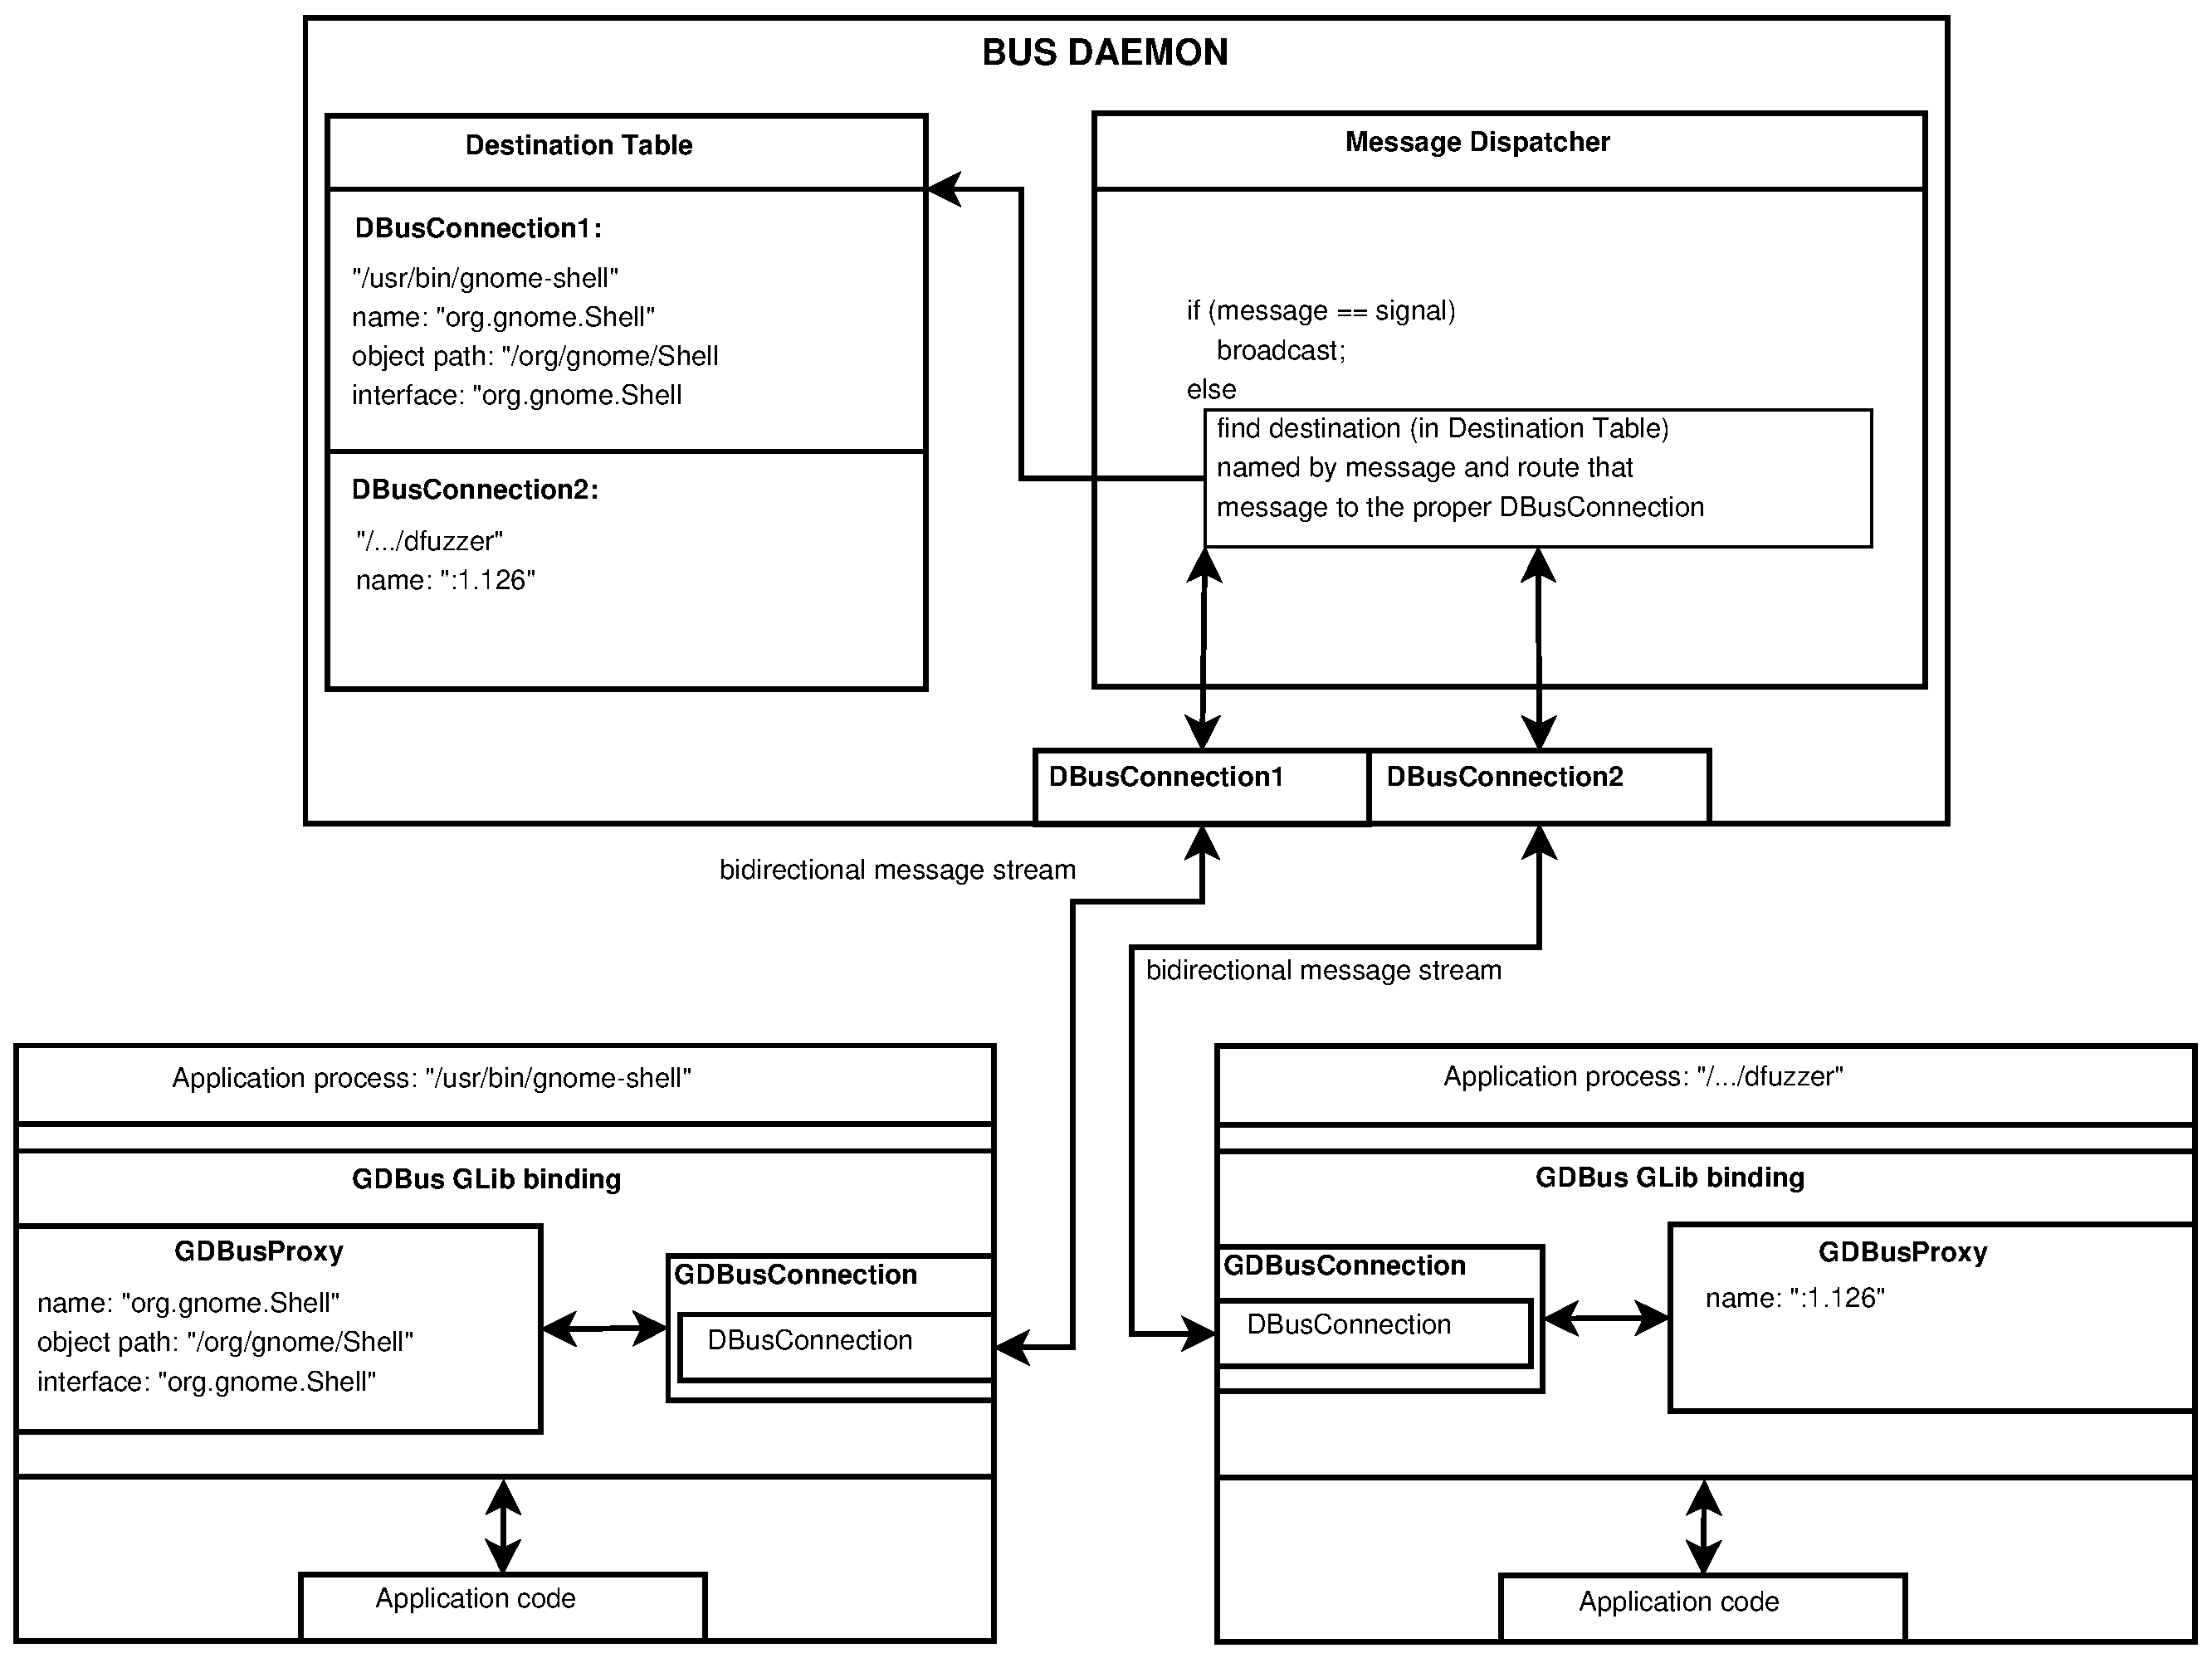
\includegraphics[width=1\textwidth]{fig/dfuzzer_diagram.eps}
\end{figure}


Before fuzz testing of~a~specified process, object introspection must be done
first. The~interface \texttt{org.freedesktop.DBus.Introspectable} contains
the~\texttt{Introspect} method which can be called using a~\texttt{GDBusProxy} object
to~get an~XML file containing all of~the~interfaces and~the~methods of~a~process
specified by~a~\texttt{GDBusProxy} object. Returned XML file is in~string format
and~so it is parsed into~a~\texttt{GDBusNodeInfo} structure which can be used
to~find a~particular interface. Interfaces are stored in~a~list
of~\texttt{GDBusInterfaceInfo} structures which contain lists
of~methods~(\texttt{GDBusMethodInfo} structure) and~to~each method there is a~list
of~its arguments~(\texttt{GDBusArgInfo} structure). The~\emph{introspection module}
which is part of~dfuzzer encapsulates all object introspection details and~provides
an~interface for~easy iteration through methods and~their arguments.\\


Every method argument signature is specified by~its
direction which is either ``out'' (returned argument signature) or
``in''~(accepted argument signature). When an~object introspection of~a~specified
interface is done, dfuzzer iterates through interface methods. For~every method,
its accepted arguments signatures~(with~direction ``in'') and a~method name are
passed to~the~\emph{fuzz module}.
Fuzz testing of~a~method passed to~the~\emph{fuzz module} takes place in~the~cycle
by~calling this method many times, but with~different arguments. Before each
call of~a~method, its arguments must be generated first. Arguments are generated
by~calling functions from~the~\emph{random module} according to~argument signature.
Generated arguments are stored in~\texttt{GVariant} types. A~\texttt{GVariant}
is used instead of~the~C \texttt{union} type as any data described
by~a~signature~(\ref{tab:tab1}) can be stored inside it. A~\texttt{GVariant} is
created by~calling the~function \texttt{g\_variant\_new()} which can be think
of~as an~analogue to~the~\texttt{sprintf()} function. The~\texttt{g\_variant\_new()}
function takes a~format string containing signatures~(\ref{tab:tab1}) as its first
argument and~remaining arguments of~the~function are sources of~data according
to~a~format string.\\

Before calling a~method, a~\texttt{GVariant} type containing structure with~all
arguments must be created. A~function call to~create this \texttt{GVariant} must
be constructed dynamically, during runtime of~dfuzzer as every method has different
number and~type of~arguments. The~\texttt{libffi} library is used for~this dynamic
function call construction. After a~\texttt{GVariant} containing structure with~all
arguments is created, a~method can be called through a~\texttt{GDBusProxy} object
using the~\texttt{g\_dbus\_proxy\_call\_sync()} function. A~method is called
synchronously because when error occurs, it returns a~\texttt{NULL} and~so dfuzzer
knows that well-known name is no longer on~the~bus daemon or no response returned
after timeout~(even if a~method has no return value, a~``method return'' message
is still sent to~the~caller). When the~\texttt{g\_dbus\_proxy\_call\_sync()}
function returns \texttt{NULL} on~a~method call, dfuzzer looks into a~tested
process status file \texttt{/proc/pid/status} to~be sure that a~tested process
really crashed. If not, it means that a~tested process spent a~long time processing
the~data received from~dfuzzer and~so it did not responded to~the~method call
from~dfuzzer in~given timeout. When dfuzzer finds out that a~tested process did
not crash, testing is continuing.\\

In~the~case a~tested process crashed or exceeded a~specified memory limit,
a~log is added to a~log file describing a~specified event. A~log file entry
is a~name of~a~method with~its arguments. If some event occured during testing
a~method, a~log is created within~a~method entry. Log headers are written in~brackets
with~a~method name as prefix and~have a~serial number~(\texttt{[method\_name LOG 1],
[method\_name LOG 2], etc.}). After a~log header there is a~message describing
an~event which occurred followed by~a~process memory size. The~last items in~log
are the~inputs on~which an~event occured and~so the~arguments signatures
with~the~corresponding values. An~example of~the~truncated log file from~fuzz
testing the~\emph{GNOME Shell 3.6.3.1}~\cite{GNOMEShell}:
\newpage
\begin{lstlisting}[frame=single]
===========================================================================
fuzzing method Eval(s):

end of fuzzing of method 'Eval'
===========================================================================
===========================================================================
fuzzing method ScreenshotArea(i, i, i, i, b, s):
[ScreenshotArea LOG 1]
  process disconnected from D-Bus
  last known process memory size: [289028 kB]
  on input:
  --i-- '2147483647'
  --i-- '2147483647'
  --i-- '2147483647'
  --i-- '-2147483648'
  --b-- 'true'
  --s [length: 67 B]-- '}>;VhlC) H-C}zF>\!550d-%49!Nax;_4S3|@W$>|1aw)%4e#
Iz4/%9@;7l|0%]BXm?'

end of fuzzing of method 'ScreenshotArea'
===========================================================================
===========================================================================
fuzzing method ScreenshotWindow(b, b, b, s):

end of fuzzing of method 'ScreenshotWindow'
===========================================================================
...
\end{lstlisting}


The~\emph{random module} provides functions for~generation of~all basic data
types~(stated in~table \ref{tab:tab1}) except arrays, structures and~dictionaries
which were not implemented.
When generating numbers, the~\texttt{rand()} and~\texttt{random()} functions are
used. Besides pseudo-random numbers, the~\emph{random module} also generates
a~specific boundary values of~number types~(also negative for~signed number types).
As dfuzzer uses GDBus binding, the~functions in~the~\emph{random module} generate
only valid UTF-8 strings. Pseudo-random characters which are used to~fill strings
are counted to~fit the~printable range:
\begin{verbatim}
        rand() % (127 - 32) + 32
\end{verbatim}
The~\emph{random module} also provides the~\texttt{NULL} terminated array of~strings,
which will be sent to~a~tested process if it has any string parameters. Tester
can include any valid UTF-8 strings inside this array including shell commands,
bus names, object paths, interfaces or format strings.\\

To~test dfuzzer functionality during an~implementation, a~test server was
implemented which exports a~well-known name on~the~session bus daemon with~one own
interface and~one method. Source codes of~dfuzzer including the test server which
was used for~its testing can be found on~\url{https://github.com/matusmarhefka/dfuzzer}.



%==============================================================================|
\chapter{Fuzz testing results}
dfuzzer was used to~fuzz test three chosen applications which use D-Bus system
for~inter-process communication:

\begin{itemize}
	\item \emph{\textbf{GNOME Shell}}~\cite{GNOMEShell} -- the~core user interface
		of~the~GNOME desktop environment providing basic functionality like
		switching between windows and~launching applications
	\item \emph{\textbf{IMSettings}}~\cite{IMSettings} -- a~framework that delivers
	Input Method settings and~applies the~changes immediately, so it will takes
	an~effect without~restarting applications and~the~desktop
	\item \emph{\textbf{Evince}}~\cite{GNOMEEvince} -- a~document viewer
		for~multiple document formats
\end{itemize}
Each application was fuzz tested twice. The~results of~testing can be found
in~log files on~the~CD.


\section{Fuzz testing \emph{Evince}}
dfuzzer was fuzz testing methods of:
\begin{verbatim}
           bus name:  org.gnome.evince.Daemon
        object path:  /org/gnome/evince/Daemon
          interface:  org.gnome.evince.Daemon
\end{verbatim}
The~first and~the~second fuzz tests results of~the~tool did not find any
non-standard behaviour of~the~\emph{Evince} document viewer.


\section{Fuzz testing \emph{GNOME Shell}}
Fuzz tests results of~the~\emph{GNOME Shell} are presented
in~the~tables~\ref{tab:tab2} and~\ref{tab:tab3}. dfuzzer was fuzz testing
methods of:
\begin{verbatim}
           bus name:  org.gnome.Shell
        object path:  /org/gnome/Shell
          interface:  org.gnome.Shell
\end{verbatim}
\newpage
The~first fuzz tests of~the~\emph{GNOME Shell} took approximately 4~minutes
and~40~seconds to~complete. The~second fuzz tests were not finished completely
because the~\emph{GNOME Shell} could not even reload from~the~crash.\\


\FloatBarrier
\begin{table}[h!]
\catcode`\-=12
\caption{Results of~first fuzz tests of~the~\emph{GNOME Shell}}
\label{tab:tab2}
\begin{center}
	\begin{tabular}{| l | l | c |}
	\hline
	\textbf{Method name} & \textbf{Event} & \textbf{Memory size [kB]} \\ \hline
	Eval(s) & -- & standard \\ \hline
	ScreenshotArea(i, i, i, i, b, s) & process disconnected from D-Bus & 146160 \\ \hline
	ScreenshotWindow(b, b, b, s) & -- & standard \\ \hline
	Screenshot(b, b, s) & -- & standard \\
	FlashArea(i, i, i, i) & -- & standard \\
	\hline
	\end{tabular}
\end{center}
\end{table}
\FloatBarrier


The~first fuzz tests results~(in table~\ref{tab:tab2}) show that a~method
\texttt{ScreenshotArea} caused a~crash of~the~\emph{GNOME Shell}. The~input
arguments were:
\begin{verbatim}
ScreenshotArea(i, i, i, i, b, s):
  --i-- '2147483647'
  --i-- '2147483647'
  --i-- '2147483647'
  --i-- '-2147483648'
  --b-- 'false'
  --s [length: 114 B]-- '\fR3~,jc5?\_FzmxB%NaO?HmnW)3e+LBq~Rn,=R>]/z
!(iyJnE);dQ*P'0cl;0,*-_x6|HQWULX]6O%"t/;V`E(dRkQmy^w';n:87kmi8CDLsJNeVi'
\end{verbatim}
Other methods did not cause any non-standard behaviour.\\\\


\FloatBarrier
\begin{table}[!h]
\catcode`\-=12
\caption{Results of~second fuzz tests of~the~\emph{GNOME Shell}}
\label{tab:tab3}
\begin{center}
	\begin{tabular}{| l | l | c |}
	\hline
	\textbf{Method name} & \textbf{Log message} & \textbf{Memory size [kB]} \\ \hline
	Eval(s) & -- & standard \\ \hline
	ScreenshotArea(i, i, i, i, b, s) & process disconnected from D-Bus & 287300 \\ \hline
	ScreenshotWindow(b, b, b, s) & process disconnected from D-Bus & 58040 \\
	\hline
	\end{tabular}
\end{center}
\end{table}
\FloatBarrier


The~second fuzz tests~(in~table~\ref{tab:tab3}) crashed the~\emph{GNOME Shell}
again with~the~following input arguments of~the~method \texttt{ScreenshotArea}:
\begin{verbatim}
ScreenshotArea(i, i, i, i, b, s):
  --i-- '-2147483648'
  --i-- '2147483647'
  --i-- '2147483647'
  --i-- '2147483647'
  --b-- 'true'
  --s [length: 164 B]-- 'PQbnvwe2FJY4UQ_E2Ei!O g"\0i"TTk%'Kp}CV-j}c~
S2\vD"`EO]-N::8:nm&ptQaoq5|Y4`Vdo0[4/9V[v`+2zCLi1OZ#}9roNlG_JzE:+!N:
;%v/b">]BgDQ7{T55E#d2GD]BfwMhDd!F[0*ZOd}7*LO&!a<Ca}V)'
\end{verbatim}
Compared to~the~first fuzz tests, one more serious crash of~the~\emph{GNOME Shell}
on~a~call of~the~method \texttt{ScreenshotWindow} was found. The~crash happened
immediately after the~\emph{GNOME Shell} restart which was caused by~the~previous
call of~the~\texttt{ScreenshotArea} method. The~method \texttt{ScreenshotWindow}
was called with~these input arguments:
\begin{verbatim}
ScreenshotWindow(b, b, b, s):
  --b-- 'false'
  --b-- 'true'
  --b-- 'false'
  --s [length: 77 B]-- 'G1C!HhBR}Id{mEU~C(8\tR)='~.|6%`Z6"[^j}.eGr_5
851X;I60x<N}8YzN^Y)t[aPC_^*'Of:d{'
\end{verbatim}
and~caused a~crash of~the~\emph{GNOME Shell} from~which it could not reload
and~only offered a~logout option.


\section{Fuzz testing \emph{IMSettings}}
Fuzz tests results of~the~\emph{IMSettings} are presented
in~the~tables~\ref{tab:tab4} and~~\ref{tab:tab5}.
dfuzzer was fuzz testing methods of:
\begin{verbatim}
           bus name:  com.redhat.imsettings
        object path:  /com/redhat/imsettings
          interface:  com.redhat.imsettings
\end{verbatim}


\FloatBarrier
\begin{table}[h!]
\catcode`\-=12
\caption{Results of~first fuzz tests of~the~\emph{IMSettings}}
\label{tab:tab4}
\begin{center}
	\begin{tabular}{| l | l | c | c |}
	\hline
	\textbf{Method name} & \textbf{Log message} & \textbf{Initial} & \textbf{Current} \\
	& & \textbf{mem. [kB]} & \textbf{mem. [kB]} \\ \hline
	GetInfoVariants(s) & memory size exceeded set limit & 4000 & 36044 \\ \hline
	GetInfoVariant(s, s) & process disconnected from D-Bus & 4000 & 83604 \\ \hline
	GetUserIM(s) & memory size exceeded set limit & 3604 & 32580 \\ \hline
	GetSystemIM(s) & memory size exceeded set limit & 3604 & 97408 \\ \hline
	IsSystemDefault(s, s) & memory size exceeded set limit & 3604 & 144064 \\ \hline
	IsUserDefault(s, s) & memory size exceeded set limit & 3604 & 178972 \\ \hline
	IsXIM(s, s) & process disconnected from D-Bus & 3604 & 214936 \\ \hline
	SwitchIM(s, s, b) & process disconnected from D-Bus & 4000 & 4060 \\ \hline
	LoadModule(s) & -- & standard & standard \\ \hline
	UnloadModule(s) & -- & standard & standard \\
	\hline
	\end{tabular}
\end{center}
\end{table}
\FloatBarrier


The~first fuzz tests results indicate that the~\emph{IMSettings} daemon is leaking
memory as can be seen from~the~table~\ref{tab:tab4}. dfuzzer also registered three
crashes of~the~\emph{IMSettings} daemon. After few calls of~the~method
\texttt{GetInfoVariants} the~\emph{IMSettings} daemon memory size reached
the~36044~kB~(the~initial memory size was 4000~kB). The~first crash occured
on~a~call of~the~method \texttt{GetInfoVariant} with~the~size of~memory 83604~kB.
The~fuzz tests of~the~next methods to~the~\texttt{IsUserDefault} method confirm
memory leaks in~the~\emph{IMSettings} daemon~(memory size raised from~the~3604~kB
to~the~178972~kB). The~last two crashes of~the~\emph{IMSettings} daemon are caused
by~the~\texttt{IsXIM} and~the~\texttt{SwitchIM} methods. The~inputs which are
responsible for~the~memory leaks and~the~crashes of~the~\emph{IMSettings} daemon
were long strings, usually with~size of~several hundreds of~bytes. These inputs
can be found in log files on~CD.\\

The~second fuzz tests~(stated in~table~\ref{tab:tab5}) confirmed the~results
of~the~first tests. Each of~the~two fuzz tests took approximately 8~minutes
to~complete.\\


\FloatBarrier
\begin{table}[h!]
\catcode`\-=12
\caption{Results of~second fuzz tests of~the~\emph{IMSettings}}
\label{tab:tab5}
\begin{center}
	\begin{tabular}{| l | l | c | c |}
	\hline
	\textbf{Method name} & \textbf{Log message} & \textbf{Initial} & \textbf{Current} \\
	& & \textbf{mem. [kB]} & \textbf{mem. [kB]} \\ \hline
	GetInfoVariants(s) & memory size exceeded set limit & 3652 & 32924 \\ \hline
	GetInfoVariant(s, s) & process disconnected from D-Bus & 3652 & 82832 \\ \hline
	GetUserIM(s) & memory size exceeded set limit & 3600 & 32500 \\ \hline
	GetSystemIM(s) & memory size exceeded set limit & 3600 & 97388 \\ \hline
	IsSystemDefault(s, s) & memory size exceeded set limit & 3600 & 145408 \\ \hline
	IsUserDefault(s, s) & memory size exceeded set limit & 3600 & 177340 \\ \hline
	IsXIM(s, s) & process disconnected from D-Bus & 3600 & 212400 \\ \hline
	SwitchIM(s, s, b) & process disconnected from D-Bus & 3645 & 3852 \\ \hline
	LoadModule(s) & -- & standard & standard \\ \hline
	UnloadModule(s) & -- & standard & standard \\
	\hline
	\end{tabular}
\end{center}
\end{table}
\FloatBarrier



%==============================================================================|
\chapter{Conclusion}
The~goal of~this work was to~use the~fuzzing for~testing applications using D-Bus
communication system and~an~automation of~this task. The~work describes existing
fuzzers for~individual testing targets and~also D-Bus communication system including
its architecture. Subsequently, the~tool architecture and~implementation are
discussed followed by~the~tests results produced by~the~implemented tool.\\

The~implemented tool~(dfuzzer) was used to~test three chosen applications --
\emph{GNOME Shell}, \emph{IMSettings} and~\emph{Evince}. An~object introspection
was used to~allow dfuzzer to~``study'' application object interfaces, so
the~tool can be used to~test all the~applications connected to~the~session bus
daemon besides ones chosen for~the~testing in~this work. The~only limitation
in~this fuzz testing automation is that some functions containing more complex
arguments~(like structures, arrays of~types and~dictionaries) are impossible
to~test with~dfuzzer, because the~author did not manage to~find the~appropriate
automated method for~generation of~such complex types during the~tool implementation.
The~current implementation of~dfuzzer skips the~functions containing complex
types~(example of~a~complex type may be an~array of~structures containing an~array
of~strings~(``\texttt{a(as)}'')). The~absence of~complex types generation should
be eliminated in~a~further development of~the~project.\\

The~testing of~chosen applications revealed bugs which were reported
to~the~developers of~the~applications. The~most bugs have been found
in~the~\emph{IMSettings} daemon which suffered from~the~crashes and~memory leaks.
These bugs were reported on~the~\emph{IMSettings Issues} page\footnote{\url{https://bitbucket.org/tagoh/imsettings/issue/1/imsettings-d-bus-interface}}, but they have
not been confirmed yet. The~\emph{GNOME Shell} tests also revealed bugs. One test
case caused the~\emph{GNOME Shell} to~crash, but it reloaded and~testing continued.
The~second test case on~the~other hand crashed the~\emph{GNOME Shell} immediately
after the~first test case and~caused that it was unable to~reload, only logout
option was offered. The~approach of~the~GNOME developers to~the~reported
bugs\footnote{\url{https://bugzilla.gnome.org/show_bug.cgi?id=699752}} was lax.
One of~them commented that the~values given to~the~tested methods are not valid,
so it is almost legit the~\emph{GNOME Shell} crashes in~this case and~that
the~tested methods are in~a~private interface used only by~certain GNOME
applications. These facts may be true, but still letting the~application to~crash
is not a~good programming practice as one of~the~developers also admitted.
The~decision wheter the~GNOME developers correct these bugs and~make
the~\emph{GNOME Shell} more robust is anyway on~them. This work is not going
to~discuss or disprove the~GNOME developers opinions, its goal was just
to~pinpoint such cases that force applications to~behave incorrectly.\\

The~implemented fuzzer is not bound to~any specific application. It targets
all the~applications connected to~the~session bus daemon, and~so its effectiveness
might not be the~same as for~a~fuzzer targeting a~specific application.
For~the~future, it would be good to~add a~generation of~complex argument types,
extend dfuzzer to~work also for~the~system bus daemon applications testing
and~also include dfuzzer into~some application test suites.


%=========================================================================
